\chapter{ESPECIFICAÇÃO DO EXPERIMENTO} % (fold)
\label{cha:especificacao_do_experimento} % (fold)

\section{Descrição do Experimento}
\label{cha:descricao_do_experimento}

Foi realizado um experimento com 60 pessoas, que se cadastraram e formaram uma rede social disposta em 12 grupos de 5 amigos. O sistema de recomendação utiliza essa rede social para obter as informações de relações de amizade entre os usuários. Neste contexto, um usuário é considerado amigo do outro quando eles pertencem a um mesmo grupo de amigos. Os grupos de usuários foram definidos a partir do envio de um e-mail com um convite de um usuário já cadastrado no sistema a outra pessoa. Este e-mail possuía um endereço de cadastro onde foi possível a pessoa se cadastrar e automaticamente já fazer parte do grupo de amigos do usuário que a convidou.

Os usuários receberam recomendações dos seus amigos e de outras pessoas presentes na rede. Além disso, as informações de avaliações de produtos por parte dos usuários foram utilizadas pelo sistema de recomendação para recomendar outros produtos a eles. Como já citado no capítulo ~\ref{cha:introducao}, foram utilizados 3 tipos de algoritmos pelo sistema de recomendação:

\begin{itemize}
  \item Baseado em similaridade entre perfis
  \item Baseado em similaridade de produtos
  \item Baseado em confiança
\end{itemize}

Inicialmente 12 pessoas foram convidadas a participar do experimento. Cada uma destas convidou outras 4 pessoas para formarem um grupo de amigos. Sendo assim, formaram-se 12 grupos de 5 amigos, totalizando 60 pessoas. Cada participante de um grupo de amigos concorda em ser definido como amigo de todos no grupo, ou seja, todas as pessoas pertencentes a um mesmo grupo de amigos se conhecem e se consideram amigas. Cada participante do experimento recebeu, leu e assinou uma cópia do Termo de Consentimento Livre e Esclarecido (vide Apêndice~\ref{cha:TCLE}) concordando em participar do experimento.

Os participantes realizaram o cadastro informando os seguintes dados pessoais:

\begin{itemize}
  \item Nome
  \item Sexo
  \item Faixa etária (18-25, 26-30, 31-40, +40)
  \item Foto
\end{itemize}

O experimento consistia em 6 etapas, onde os participantes deveriam executar tarefas descritas no próprio sistema.

\subsection{Primeira Etapa}
\label{cha:primeira_etapa}

Logo após a finalização do cadastro no sistema, a primeira etapa do experimento era iniciada. Ela consistia na avaliação de 20 produtos em comum a todos os participantes de todos os grupos. Esses produtos foram selecionados previamente, com o intuito de abranger os diferentes gostos de todos os participantes. Esta etapa foi necessária para que houvesse um \textit{rating overlap} no sistema, ou seja, para que todos os usuários avaliassem um mesmo conjunto de produtos. Com isso, foi possível calcular a similaridade de perfis entre todos os participantes da rede. Além disso, com esta etapa, resolve-se o problema dos \textit{coldstart users}, pois todos os usuários iniciam o uso do sistema ativamente.

Avaliar um produto significa dizer o quanto o participante considera aquele produto como relevante para si, ou seja, o quanto ele se interessa pelo produto. A avaliação é feita por meio da atribuição de uma nota de 1 a 5, sendo que 1 significa ausência de interesse e 5 representa muito interesse. Esse interesse não significa necessariamente uma atitude de compra. O objetivo dessa avaliação é saber realmente o interesse do participante, podendo representar cobiça ou curiosidade, além de admiração pelo produto. A interface de avaliação está apresentada na Figura~\ref{fig:product-rating}.

\begin{figure}[htp]
  \centering
  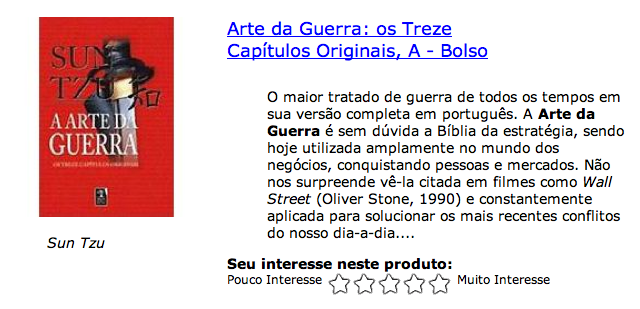
\includegraphics[width=\textwidth]{imagens/product-rating}
  \caption{\it Apresentação de produto para avaliação do usuário}
  \label{fig:product-rating}
\end{figure}

Caso o participante não conhecesse o produto na hora de avaliá-lo, ou seja, não tivesse ouvido falar dele ou não tivesse conhecimento suficiente para reconhecê-lo, até o instante em que ele lhe foi apresentado, ele deveria informar isso ao sistema por meio de uma opção disponibilizada após a avaliação de cada produto. Mesmo não conhecendo, o participante avaliava o produto de acordo com o seu grau de interesse. Neste caso, a avaliação deveria ser feita apenas com base na foto e descrição do produto.

\subsection{Segunda Etapa}
\label{cha:segunda_etapa}

Ao finalizar a primeira etapa, automaticamente a segunda etapa era ativada. Esta visava conhecer os interesses particulares dos participantes. Para isso, foram disponibilizados vários produtos, separados nas diversas categorias, sendo que o participante deveria avaliar 10 produtos. As categorias escolhidas foram as seguintes:

\begin{itemize}
  \item CDs
  \item DVDs e Blu Ray
  \item Livros
  \item Livros Importados
  \item Celulares e Telefonia Fixa
  \item Vinhos e Bebidas
  \item Relógios e Presentes
  \item Informática e Acessórios
\end{itemize}

Os dados dos produtos foram retirados do site da Submarino\footnote{http://www.submarino.com}, sendo que apenas algumas categorias de livros, CDs e DVDs foram cadastradas no sistema e apenas os 60 produtos mais vendidos das outras categorias foram inseridos no cadastro.

Uma busca por nome foi implementada para que os participantes pudessem localizar um produto ao seu gosto e avaliá-lo. Nesta etapa, também estava disponível a opção de ``Não conheço'', pois era possível o participante encontrar durante a busca um produto desconhecido que o agradasse. A interface de busca de produtos está ilustrada na Figura~\ref{fig:product-search}.

Esta etapa era necessária para que os participantes avaliassem outros produtos além daqueles da primeira etapa que garantem o \textit{rating overlap}. Além dos produtos em comum, os sistemas de recomendação necessitam que as pessoas contribuam com informações individuais, pois um sistema de recomendação sempre indica produtos que não tenham sido avaliados pelo usuário que receberá a recomendação. Desse modo, além das pessoas avaliarem produtos em comum, é necessário que elas avaliem diferentes produtos para que o sistema de recomendação tenha outros produtos a indicar.

\begin{figure}[htp]
  \centering
  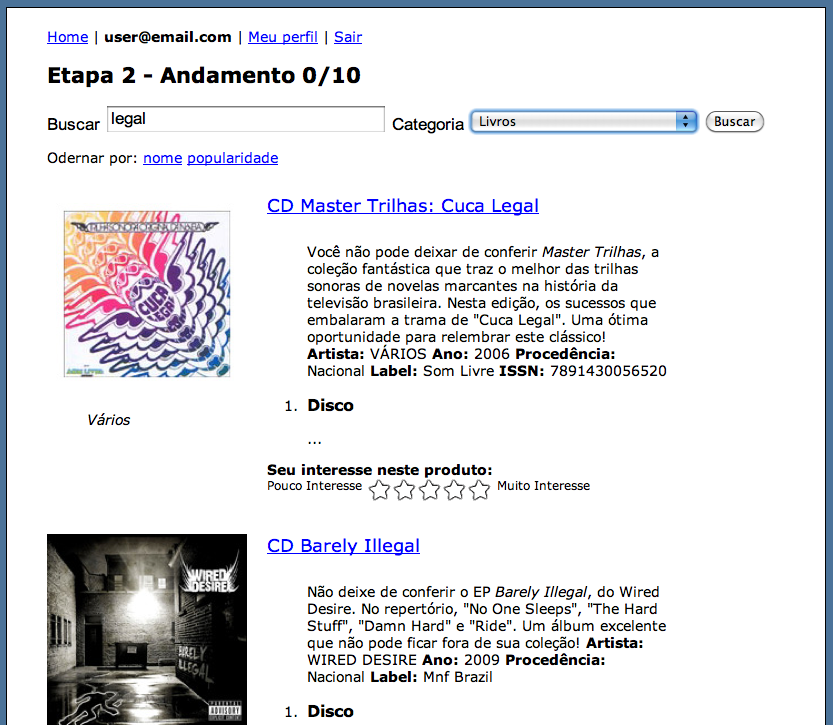
\includegraphics[width=\textwidth]{imagens/search}
  \caption{\it Interface de busca de produtos}
  \label{fig:product-search}
\end{figure}

\subsection{Terceira Etapa}

% TODO verificar tempo verbal no texto todo
Assim que todos os participantes terminassem as duas primeiras etapas do experimento, a terceira etapa era iniciada. Enquanto isso não ocorresse, quem terminava a segunda etapa recebia a mensagem do sistema informando que a terceira etapa estava desabilitada. Esse sincronismo foi necessário, pois as etapas seguintes necessitavam das informações de avaliação de produtos de todas as pessoas.

Nesta terceira etapa, o participante deveria recomendar produtos às pessoas do seu grupo. Como todos os integrantes de um grupo eram amigos entre si, era esperado que as recomendações de produtos fossem fáceis de serem realizadas, porque normalmente as pessoas conhecem os gostos dos amigos. Por isso, cada participante deveria recomendar 5 produtos a cada amigo, ou seja, 20 produtos no total.

A Figura~\ref{fig:stage-3} apresenta a interface do usuário no início da etapa 3.

A busca de produtos estava disponível nesta etapa, bem como as avaliações de todos os amigos contendo no total os 30 produtos que cada um avaliou nas duas primeiras etapas do experimento. Não era possível um participante recomendar um produto já avaliado pela pessoa que receberia a recomendação, assim como não era possível recomendar o mesmo produto mais de uma vez para a mesma pessoa. Mesmo assim, o participante poderia receber duas recomendações de um mesmo produto, desde que elas fossem feitas por amigos diferentes. Neste caso o sistema armazenava as duas recomendações como distintas e mostrava apenas uma vez o produto para ser avaliado pela pessoa que recebeu a recomendação.

\begin{figure}[htp]
  \centering
  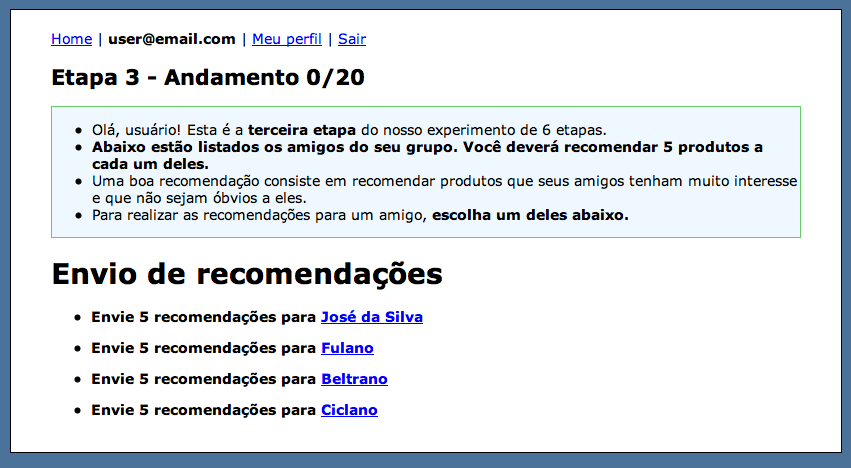
\includegraphics[width=\textwidth]{imagens/stage-3}
  \caption{\it Envio de recomendações de produtos}
  \label{fig:stage-3}
\end{figure}

Esta etapa era necessária para que posteriormente fosse possível analisar a eficiência da recomendação de produtos realizadas por amigos: nossa hipótese é que tal tipo de recomendação deveria ser mais eficiente do que as recomendações realizadas por pessoas desconhecidas ou pelo sistema de recomendação \cite{bonhard2007devil}.

\subsection{Quarta Etapa}

Depois de ter feito as 5 recomendações de produtos a cada amigo, o participante deveria recomendar alguns produtos a pessoas que não faziam parte do seu grupo, ou seja, pessoas desconhecidas. Ficava visível ao participante uma lista gerada pelo sistema contendo alguns desconhecidos. Tal lista foi gerada aleatoriamente em um aplicativo desenvolvido especialmente para este fim. Para cada pessoa na lista, o participante deveria recomendar apenas um produto. As avaliações de produtos realizadas por essas pessoas da lista ficavam disponíveis ao participante, sendo que ele deveria se basear apenas nestes dados e nos dados pessoais da pessoa para lhe recomendar um produto.

Com as recomendações realizadas por pessoas desconhecidas, foi possível comparar estas com aquelas feitas pelos amigos durante a terceira etapa do experimento. Foi necessário esperar todos os participantes terminassem a terceira e quarta etapas para que o experimento desse continuidade, já que todas essas recomendações de produtos seriam utilizadas nas etapas seguintes.

\subsection{Quinta Etapa}

A quinta etapa tinha como propósito mostrar apenas as recomendações diretas, ou seja, aquelas que foram feitas tanto pelos amigos do participante, como pelas pessoas desconhecidas. Os produtos recomendados eram listados ao participante para que ele os avaliasse novamente de acordo com o seu grau de interesse, além de informar se os conhecia ou não.

Na listagem de recomendações, não ficava visível ao participante quem lhe recomendou o produto, para que a origem da recomendação não tivesse nenhuma influência na hora de demonstrar o seu nível de interesse no produto. Caso estivesse exposto que um amigo seu lhe recomendou o produto, o participante poderia avaliá-lo bem só por causa do laço de amizade que tem com o recomendador. Ou, no caso contrário, avaliar mal um produto só porque não conhece a pessoa que o recomendou. Não havendo esse tipo de influência foi possível analisar as avaliações de produtos recomendados por amigos e desconhecidos de modo semelhante.

Para o sistema realizar as recomendações baseadas em confiança, era necessário que a terceira e quarta etapas fossem finalizadas por todos os participantes. Ao término da segunda etapa o sistema já poderia recomendar produtos, mas utilizando apenas os algoritmos baseados em perfil e em produto. A utilização desses algoritmos já era possível porque as avaliações dos 20 produtos da primeira etapa e a dos 10 da segunda já forneciam dados suficientes. Porém, como o algoritmo baseado em confiança necessita da avaliação de produtos recomendados diretamente por pessoas, foi decidido que todas as recomendações realizadas pelo sistema, a partir dos algoritmos baseados em perfil, produto e confiança, seriam realizadas ao término da quarta etapa. Com a avaliação dos produtos recomendados na terceira e quarta etapas os algoritmos baseados em perfil e em produto teriam mais dados para os seus cálculos.

Nenhum participante desistiu do experimento nesta etapa. No total, 51 participantes alcançaram a sexta e última etapa.

\subsection{Sexta Etapa}

A sexta etapa do experimento consistia na avaliação dos produtos recomendados pelo sistema aos participantes. Foram utilizados os 3 tipos de algoritmos para as recomendações, sendo que cada um deles originou 10 recomendações de produtos, totalizando 30 recomendações. Em alguns casos dois algoritmos diferentes recomendaram o mesmo produto. Quando isso ocorria, a recomendação era contabilizada normalmente para os dois algoritmos e o produto era mostrado apenas uma vez ao participante para ser avaliado.

\begin{table}
\centering
\begin{tabular}{c c c}
	\hline \hline
	\textbf{Etapa}	&	\textbf{Participantes que desistiram}	&	\textbf{Participantes que finalizaram}	\\
	\hline
	1	&	2	&	58	\\
	\hline
	2	&	2	&	56	\\
	\hline
	3	&	3	&	53	\\
	\hline
	4	&	2	&	51	\\
	\hline
	5	&	0	&	51	\\
	\hline
	6	&	1	&	50	\\
	\hline
\end{tabular}
\caption{\it Número de participantes durante as etapas do experimento}
\label{table:participantes}
\end{table}

Esta foi a etapa mais importante do experimento, pois é nela que se obteve os resultados das avaliações dos produtos recomendados com base na confiança. Além disso, houve também a avaliação dos produtos recomendados com base nos outros dois algoritmos, para que se pudesse analisar e comparar a eficiência dos três algoritmos utilizados no experimento.

Assim que os participantes terminavam as avaliações dos produtos, uma mensagem de agradecimento era mostrada e o experimento era finalizado.

Apenas um participante desistiu desta etapa final, totalizando 50 pessoas em um total de 60 a realizarem todas as etapas do experimento. A Tabela~\ref{table:participantes} mostra o número de participantes que realizaram as diferentes etapas do experimento e o número de participantes que desistiram do experimento durante as mesmas.